% fig:paths — instrumented paths (probe vs telemetry vs video vs attack UL).
\begin{tikzpicture}[
  font=\sffamily\fontsize{7.2}{8.6}\selectfont,
  >=Latex,
  endpoint/.style={
    rectangle, rounded corners=2.5pt,
    draw=ink!55, fill=boxFill, line width=0.7pt,
    align=center, inner xsep=4pt, inner ysep=3.5pt,
    minimum width=1.55cm, minimum height=1.55cm,
  },
  calloutR/.style={
    rectangle, rounded corners=2pt,
    draw=freshR, fill=freshR!8, line width=0.65pt,
    font=\sffamily\fontsize{6.4}{7.4}\selectfont,
    text=freshR, inner sep=2.8pt, align=center,
  },
  calloutG/.style={
    rectangle, rounded corners=2pt,
    draw=probeG, fill=probeG!8, line width=0.65pt,
    font=\sffamily\fontsize{6.4}{7.4}\selectfont,
    text=probeG, inner sep=2.8pt, align=center,
  },
  cotenant/.style={
    rectangle, rounded corners=2pt,
    draw=sliceA!70, fill=white, line width=0.65pt,
    align=center, inner xsep=3.5pt, inner ysep=2.8pt,
    font=\sffamily\fontsize{5.9}{6.8}\selectfont,
    minimum width=1.55cm, minimum height=1.10cm,
  },
  flow/.style={-{Latex[length=2.1mm,width=1.7mm]}, line width=1.05pt},
]

% ===================== Victim UAS (GCS + UAV), same shared slice =====================
\node[endpoint] (gcs) at (0, 3.55) {%
  
\includegraphics[height=0.62cm]{gcs_laptop}\\[1pt]
  \textbf{GCS}%
};
\node[endpoint] (uav) at (4.95, 3.55) {%
  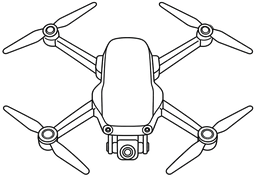
\includegraphics[height=0.62cm]{uav}\\[1pt]
  \textbf{UAV}\\[-1pt]
  {\fontsize{5.8}{6.6}\selectfont(victim UE)}%
};

\node[calloutR, left=5.5pt of gcs, align=center,
      minimum width=1.05cm, minimum height=1.05cm] (staleBox) {%
  
\includegraphics[height=0.42cm]{drone_delay}\\[0.5pt]
  state\\[-1pt]
  stale%
};

% Two lines on purpose: on one line this box is the widest node in the fit, and the
% slice outline it drags right overlaps the External DN cloud, which sits outside the
% slice. Measured: one line leaves slice.east 17 pt past dn.west, two lines leave 16 pt
% of air. Re-measure before widening this label again.
\node[calloutG, right=5.5pt of uav, align=center] (kpiBox) {%
  
\includegraphics[height=0.42cm]{kpi}\\[0.5pt]
  command-leg\\[-1pt]
  KPIs green%
};

% The leg probe is a symmetric pair, one instance per direction on its own port, so it
% is drawn as two arrows: the command leg stays healthy, the return leg is where the
% delay appears. Four flows, evenly spaced at 0.45 cm.
\draw[flow, probeG] ([yshift=0.68cm]gcs.east) -- node[above, font=\fontsize{6.2}{7.2}\selectfont, text=probeG, inner sep=0.8pt] {%
  \textbf{(1a)} Leg probe :48002 (command)%
} ([yshift=0.68cm]uav.west);

\draw[flow, freshR] ([yshift=0.23cm]uav.west) -- node[above, font=\fontsize{6.2}{7.2}\selectfont, text=freshR, inner sep=0.8pt] {%
  \textbf{(1b)} Leg probe :48003 (return)%
} ([yshift=0.23cm]gcs.east);

\draw[flow, freshR] ([yshift=-0.22cm]uav.west) -- node[above, font=\fontsize{6.2}{7.2}\selectfont, text=freshR, inner sep=0.8pt] {%
  \textbf{(2)} Delivery age $\delta$/belief%
} ([yshift=-0.22cm]gcs.east);

\draw[flow, videoP] ([yshift=-0.67cm]uav.west) -- node[above, font=\fontsize{6.2}{7.2}\selectfont, text=videoP, inner sep=0.8pt] {%
  \textbf{(3)} Video :5202%
} ([yshift=-0.67cm]gcs.east);

% No slice box here. The GCS, the UAV and the co-tenants are subscribers of ONE slice
% (Sec. III), so a single enclosure is drawn at the end, after every node exists. Two
% boxes here would reproduce the cross-slice reading the paper no longer makes.

% ===================== gNB + spokes (drawn before fh) =====================
\node[
  regular polygon, regular polygon sides=6,
  draw=gnbGrey, fill=gnbGrey!12, line width=0.85pt,
  minimum size=1.55cm, inner sep=1pt, align=center,
  font=\sffamily\fontsize{6.8}{7.8}\selectfont
] (gnb) at (2.45, 0.85) {%
  
\includegraphics[height=0.55cm]{gnb}\\[0.5pt]
  \textbf{gNB/cell}%
};

\draw[ink!55, line width=0.75pt] (gcs.south) -- (gnb.north west);
\draw[ink!55, line width=0.75pt] (uav.south) -- (gnb.north east);

% false-healthy: smaller + higher, on top of spokes
\node[
  rectangle, rounded corners=2pt, draw=muted, fill=white, line width=0.55pt,
  align=center, inner xsep=3pt, inner ysep=1.6pt,
  font=\sffamily\fontsize{5.3}{6.2}\selectfont, text=ink
] (fh) at ($(gcs.east)!0.5!(uav.west)+(0,-1.02)$) {%
  false-healthy $=$ contrast of monitors%
};

% ===================== Co-tenant UEs, same shared slice (left; gap before External DN) =====================
\node[cotenant] (r1) at (-0.05, -1.15) {%
  
\includegraphics[height=0.36cm]{ue}\\[0.5pt]
  Co-tenant UE 1%
};
\node[cotenant] (r2) at (1.75, -1.15) {%
  
\includegraphics[height=0.36cm]{ue}\\[0.5pt]
  Co-tenant UE 2%
};
\node[font=\fontsize{9.0}{10.0}\selectfont, text=sliceA] (rdots) at (2.95, -1.15) {\textbf{\ldots}};
\node[cotenant] (rN) at (4.15, -1.15) {%
  
\includegraphics[height=0.36cm]{ue}\\[0.5pt]
  Co-tenant UE $N$%
};

\node[
  cloud, cloud puffs=9, cloud ignores aspect,
  draw=muted, fill=boxFill, line width=0.7pt,
  minimum width=1.65cm, minimum height=0.88cm,
  align=center, font=\sffamily\fontsize{6.4}{7.4}\selectfont
] (dn) at (9.40, -1.15) {External DN};

\draw[flow, rogueO] (rN.east) -- (dn.west);
\node[font=\fontsize{6.2}{7.2}\selectfont, text=rogueO, below=3.5pt of dn] {%
  \textbf{(4)} Attack UL (not C2 IP)%
};

\draw[ink!55, line width=0.75pt] (gnb.south west) -- (r1.north);
\draw[ink!55, line width=0.75pt] (gnb.south) -- (r2.north);
\draw[ink!55, line width=0.75pt] (gnb.south east) -- (rN.north);

% ===================== The one shared slice =====================
% Fitted to the subscribers and the cell only. The External DN is deliberately left
% outside: it is where the adversary's traffic goes, not part of the slice.
\node[draw=sliceB, dashed, line width=0.9pt, rounded corners=6pt,
      fit=(staleBox)(gcs)(uav)(kpiBox)(gnb)(r1)(rN), inner xsep=7pt, inner ysep=9pt]
      (slice) {};
\node[font=\sffamily\bfseries\fontsize{7.0}{8.4}\selectfont, text=sliceB,
      anchor=north west, align=left, inner sep=0pt]
      at ([xshift=2pt, yshift=10pt]slice.north west)
      {Shared eMBB slice, one cell: GCS, UAV and co-tenants are ordinary subscribers of the same slice};

% ===================== Legend =====================
\node[
  rectangle, draw=muted!50, fill=boxFill, rounded corners=2pt,
  line width=0.55pt, anchor=north, inner sep=4.5pt,
  font=\sffamily\fontsize{6.0}{7.2}\selectfont
] at (2.75, -2.75) {%
  \bfseries
  \begin{tabular}{@{}l@{\hspace{0.75em}}l@{}}
  {\color{probeG}$\rightarrow$} green $=$ link monitors &
  {\color{freshR}$\leftarrow$} red $=$ freshness / belief \\[1pt]
  {\color{videoP}$\leftarrow$} purple $=$ video load (conditioner) &
  {\color{rogueO}$\rightarrow$} orange $=$ adversary (co-tenant UL) \\
  \end{tabular}%
};

\end{tikzpicture}
